\chapter{Desenvolvimento do projeto}
%Neste capitulo deve fazer uma introdução na qual são indicados os requisitos do sistema a implementar. Será uma balança, mas quais as caracteristicas da mesma ? Disso depende os componentes selecionados.
Para o desenvolvimento deste projeto, foi criado um \textit{kit} de desenvolvimento o que permitiu a realização de testes, com vista à validação do projeto, bem como à execução de alterações e melhoramentos.
\\
\\
%Qual a resolução do dispaly LCD e a Gama da celula de peso.
Analisando a \autoref{Kit_Desenvolvimento_2}, pode-se verificar a montagem em esqueleto do equipamento.
\\
\begin{figure}[H]
	\centering
	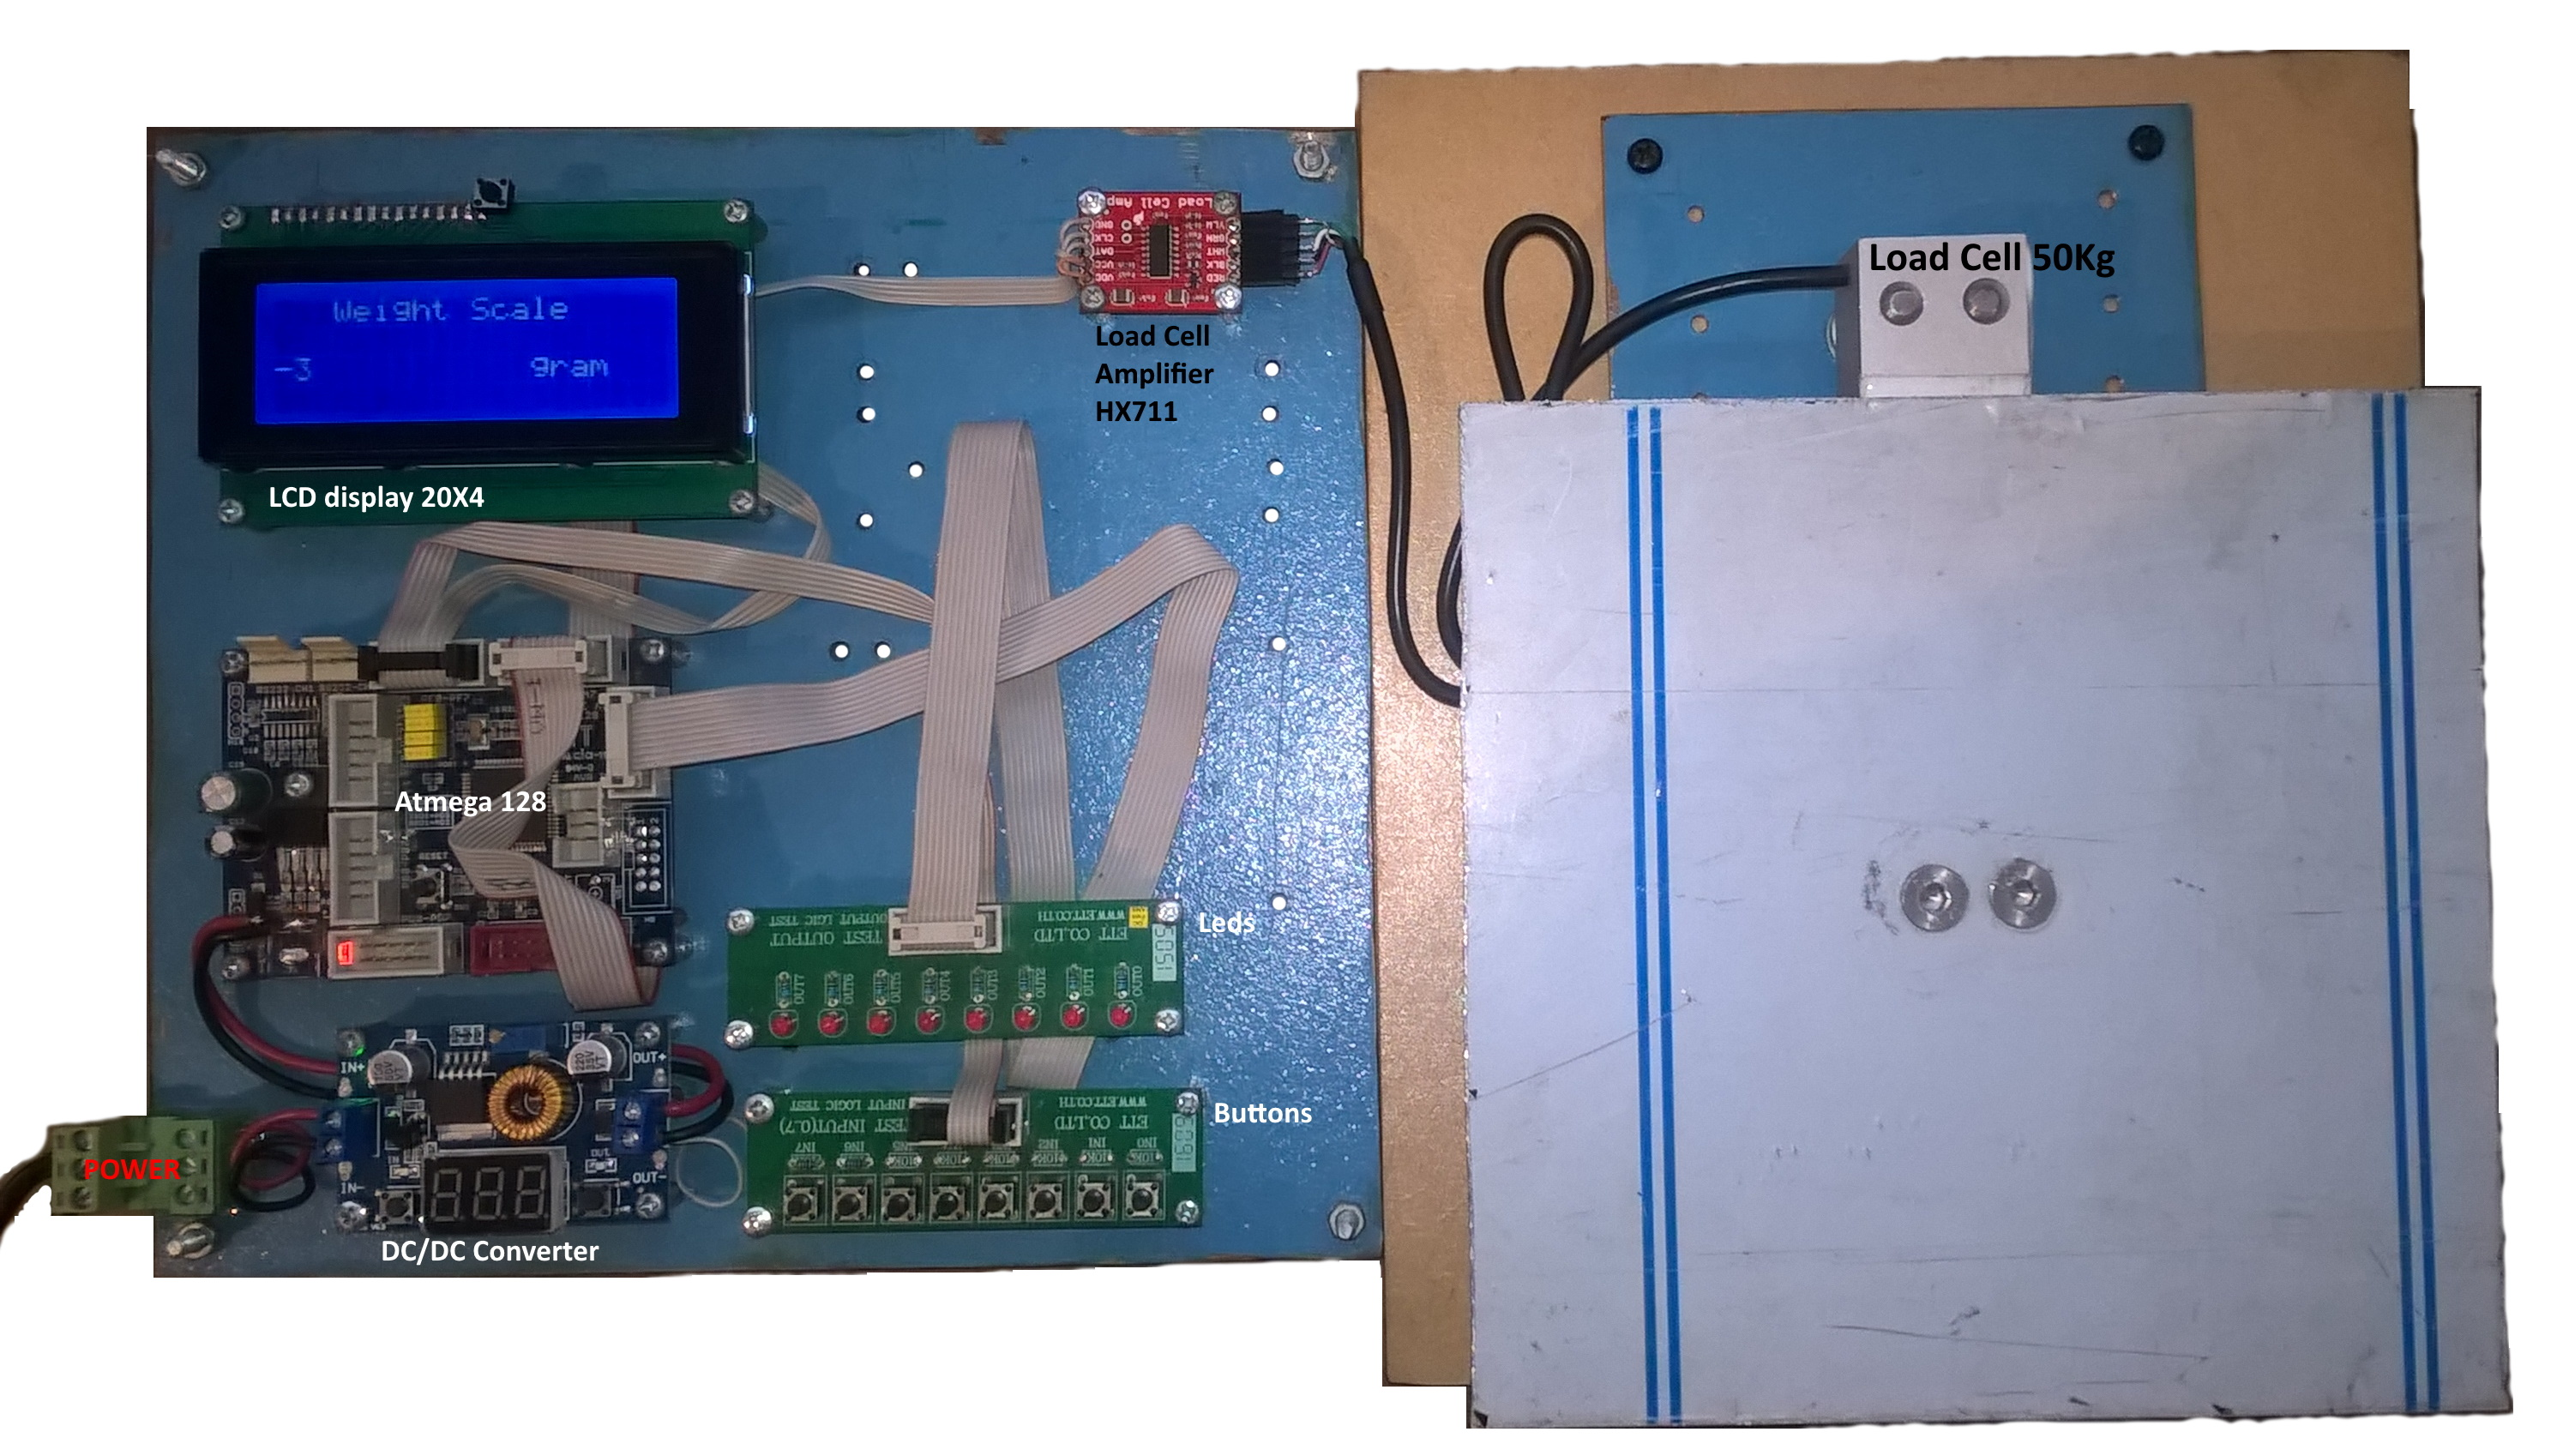
\includegraphics[scale=0.12]{./image/PESTA/kit/Kit_Desenvolvimento_2.jpg}
	\caption{Kit de Desenvolvimento}
	\label{Kit_Desenvolvimento_2}
\end{figure}
\figurespace{.5}
A seguir na \autoref{Diagrama-bloco-2} estão representados os elementos em diagrama de blocos.
\\
%Pôr a celula de caraga representada por um bloco
%comunicação série
%que tipo de comunicações ?
%O display visualiza o que ?
%O objectivo do botões e leds indicadores?
\begin{figure}[H]
	\centering
	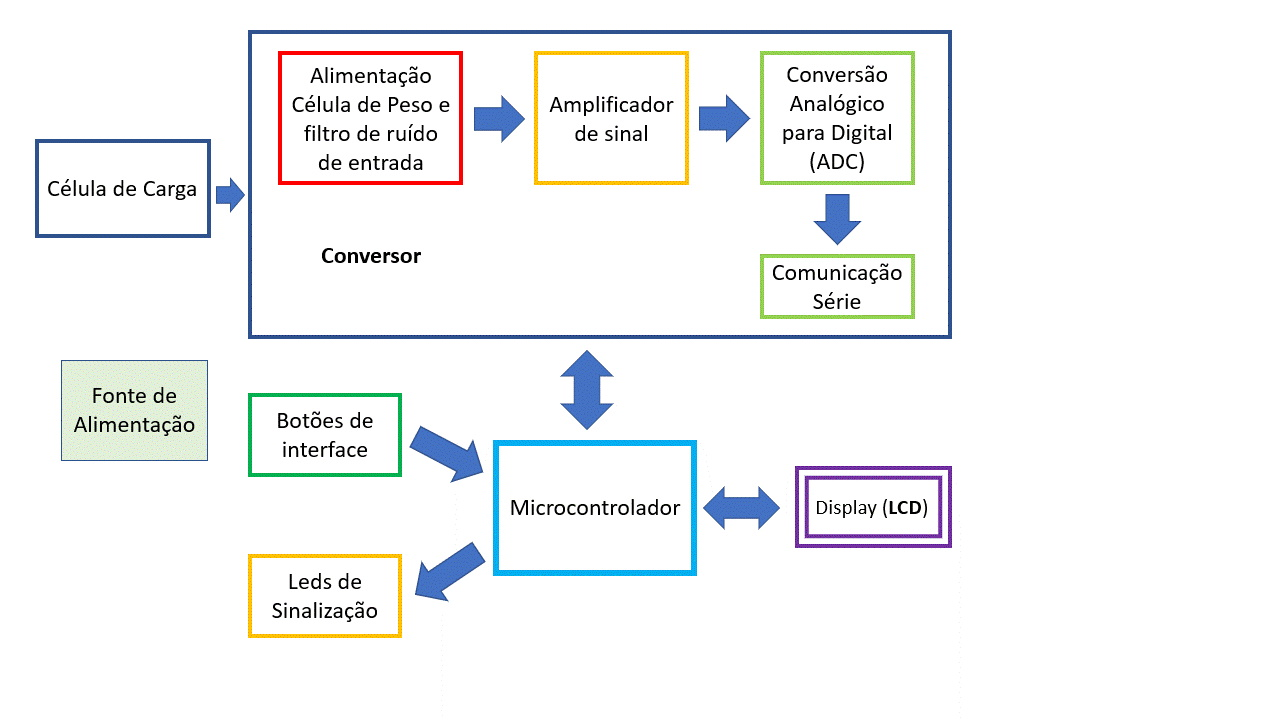
\includegraphics[scale=0.5]{./image/PESTA/Diagrama/Diagrama-bloco-2.jpg}
	\caption{Diagrama blocos do sistema implementado}
	\label{Diagrama-bloco-2}
\end{figure}
\figurespace{.5}
O microcontrolador usado neste projeto é um Atmega 128, a célula de peso é de $50 \; Kg$ com uma saída de proporção de $\; 2 \; mV/V \;$. É usado um amplificador de célula de carga com a referência HX711, que tem um protocolo de comunicação proprietário.
É utilizo um \textit{display} \acs{lcd} para visualizar os valores medidos (com a sua grandeza), e também para visualizar o fator de divisão que converte o valor lido da célula de carga pelo \acs{adc} no seu respetiva correspondente valor de massa. Os
botões são usados para saltar entre \textit{Menus} e os \acsp{led} servem como indicadores de estado, isto é, se está a usar os parâmetros \textit{default} ou de \textit{offset}.
\\
\\
Nas seguintes secções serão apresentados os componentes utilizados no projeto, assim como os aspetos relacionados com a implementação dos mesmos.
%%%%%%%%%%%%%%%%%%%%%%%%%%%%%%%%%%%%%%%%%%%%%%%%%%%%%%%%%%
\section{Célula de carga}
Para medir a massa, recorreu-se a uma célula de carga de $50 \; Kg$ (\autoref{Load_Cell_1}). Esta célula de carga utiliza sensores piezoresistivos numa montagem em ponte \textit{Wheatstone}. Esses locais são determinados pela configuração mecânica da célula de carga de forma a obter a leitura linear e proporcional ao peso exercido, isto é, ter um comportamento similar ao de uma mola.
%explicar melhor esta parte da montagem
\\
\begin{figure}[H]
	%\captionsetup{justification=raggedright,singlelinecheck=false}
	\centering
	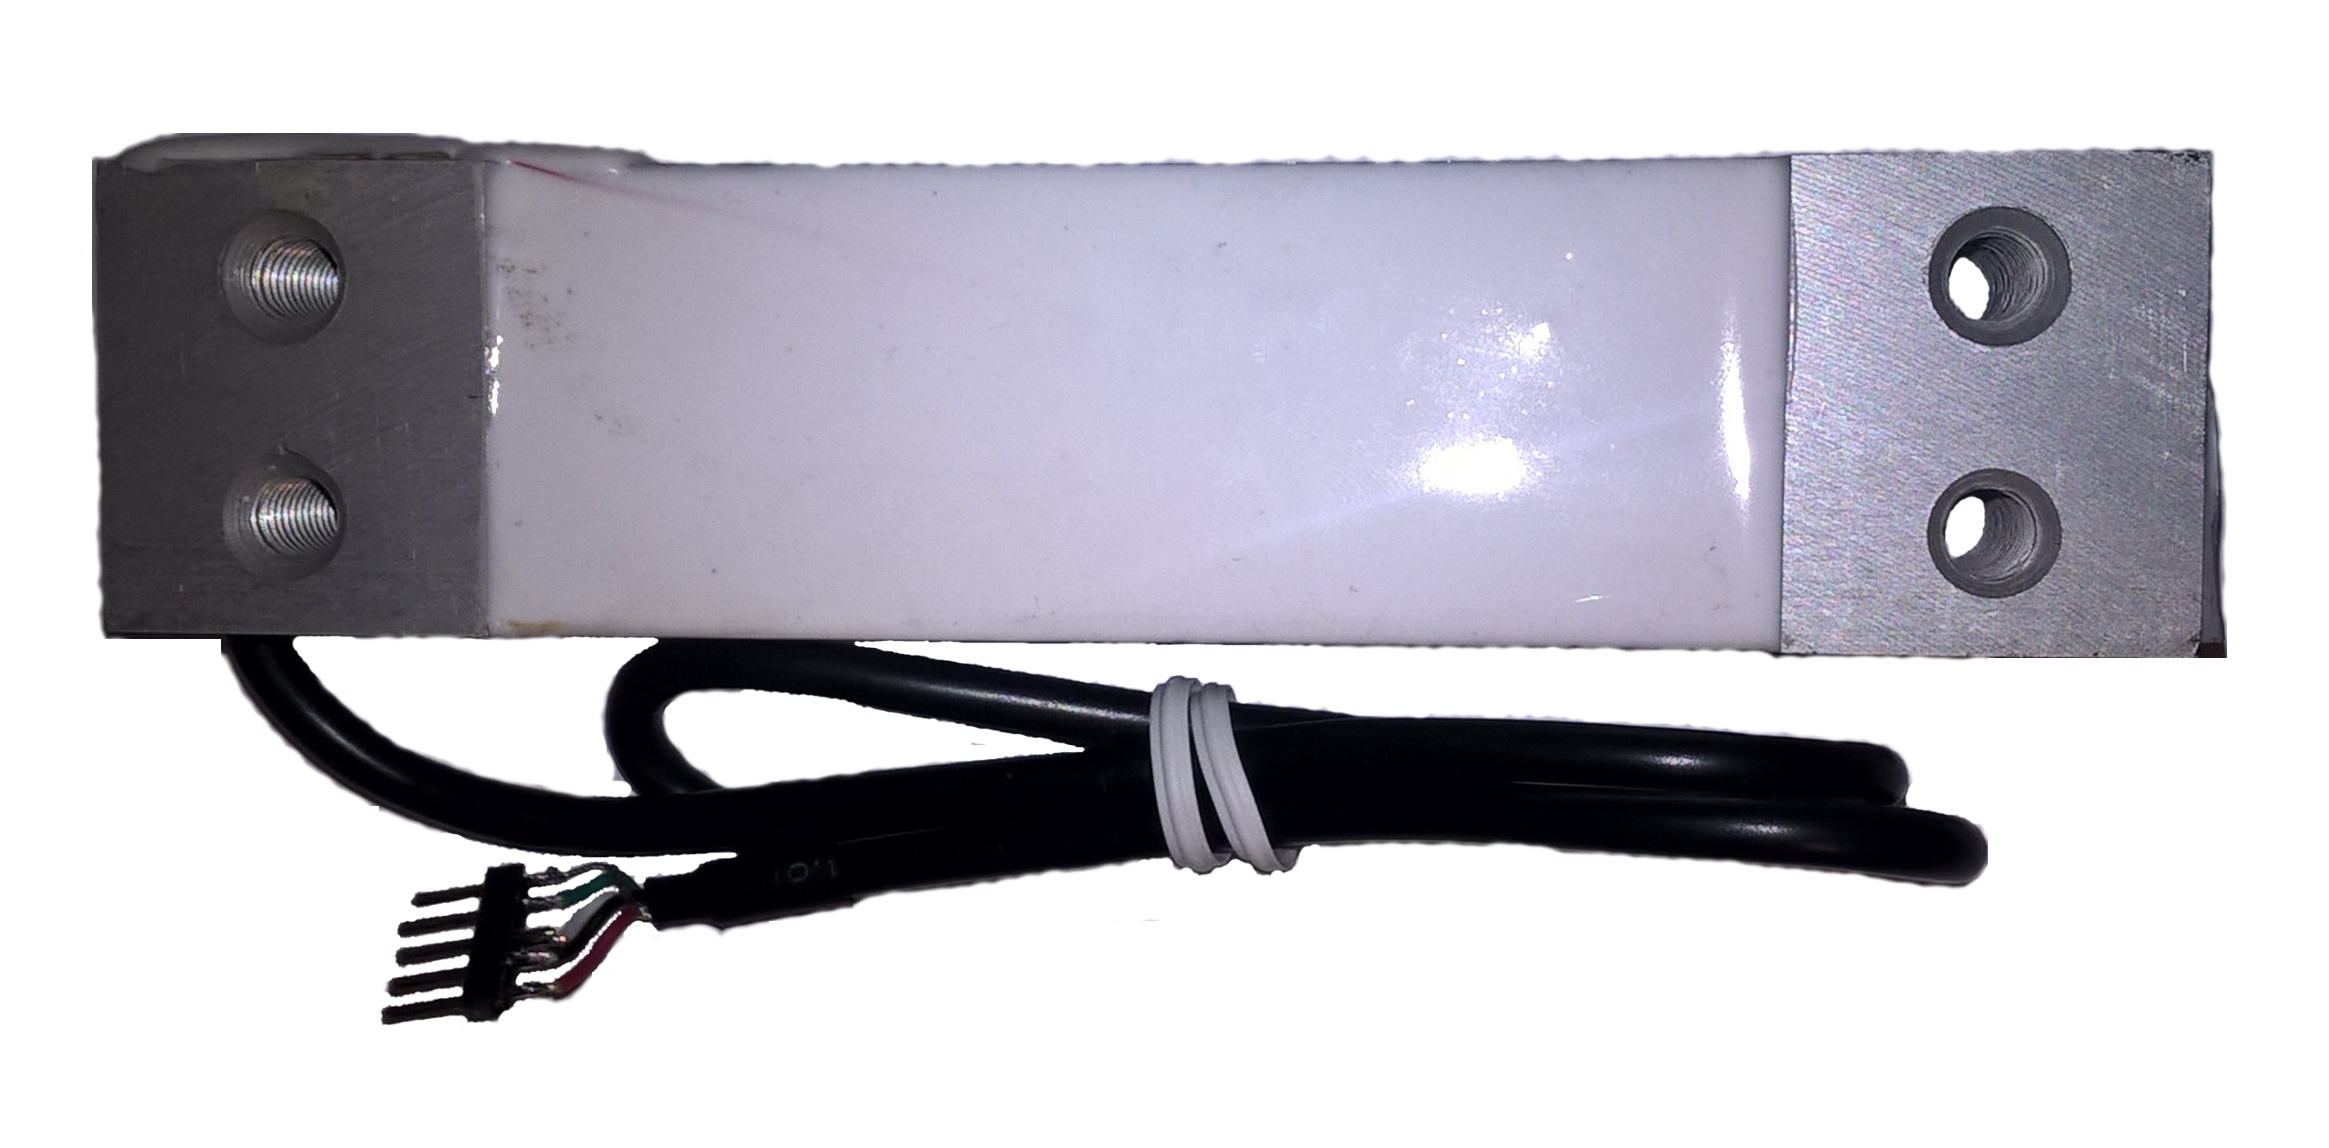
\includegraphics[scale=0.15]{./image/PESTA/material/Load_Cell_1.jpg}
	\caption{Célula de carga de $50 \; Kg$}
	\label{Load_Cell_1}
\end{figure}
\figurespace{.5}
O termo piezoresistividade deriva da palavra grega \textit{piezin}, que significa "pressionar". É um efeito exibido por vários materiais que sofrem uma mudança na resistividade devido a uma pressão aplicada. O efeito foi descoberto pela primeira vez por Lord Kelvin em 1856, que notou que a resistência dos fios de cobre e ferro aumentava quando em tensão mecânica. Ele também observou que os fios de ferro apresentavam uma alteração maior na resistência do que os de cobre. 
A primeira aplicação do efeito piezoresistivo não apareceu até à década de 1930.
\\
\\
Em vez de usar fios de metal, são geralmente feitos de uma folha de metal fina, montada numa película de suporte, que pode ser colada numa superfície. O sensor de fita de metal típico é representado na \autoref{strain_gauge_1} \cite{book-9}.
Estes sensores são implementados numa montagem do tipo ponte de \textit{Wheatstone}, de acordo com o esquema da \autoref{wheatstone-1}.
\\
\\
\begin{minipage}[!b]{.6\linewidth}
\begin{figure}[H]
	\captionsetup{justification=raggedright,singlelinecheck=false}
	\flushleft
	\figurespace{1}
	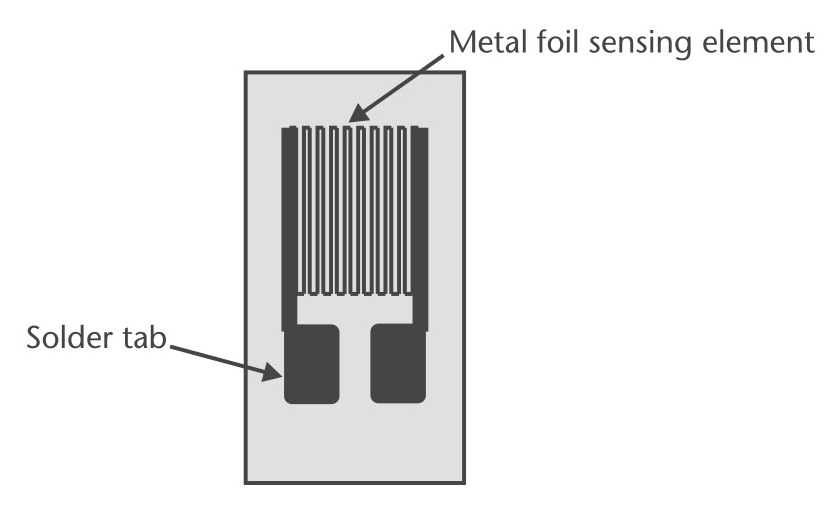
\includegraphics[height=4cm]{./image/PESTA/general/strain_gauge_1.jpg}
	\caption{Fita metálica \textit{strain gauge} \cite{book-9}}
	\label{strain_gauge_1}
\end{figure}
\end{minipage}
\begin{minipage}[!b]{.4\linewidth}
\begin{figure}[H]
	\captionsetup{justification=raggedright,singlelinecheck=false}
	\flushleft
	\vspace{1cm}
	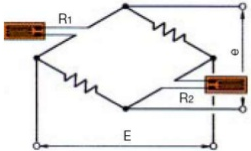
\includegraphics[height=4cm, width=4cm]{./image/PESTA/schematic/Wheatstone-1.png}
	\qquad \caption{Ponte \textit{Wheatstone}}
	\label{wheatstone-1}
\end{figure}
\end{minipage}
\minipagespace{.1}
\hspace*{1cm}\url{https://www.slideshare.net/maneeb/strain-gauge-loadcell-ppt}
%É esta a implementação utilizada no trabalho ?

%Fazer uma introdução à figura 3.6.
%Pôr sinal de massa na figura.
\vspace{.5cm}
Para uma melhor compreensão do funcionamento da ponte de \textit{Wheatstone}, a seguir é apresentado o princípio de funcionamento da ponte apenas com resistências, que está apresentada na \autoref{wheatstone-2}.
\\
\begin{minipage}[!b]{.45\linewidth}
	\begin{figure}[H]
		\captionsetup{justification=raggedright,singlelinecheck=false}
		\flushleft
		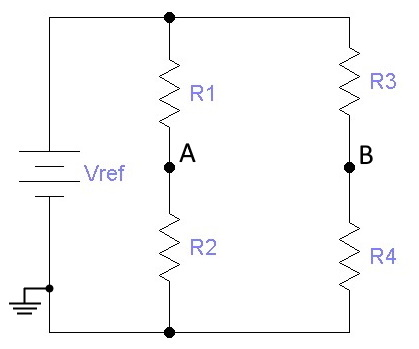
\includegraphics[height=5cm]{./image/PESTA/schematic/Wheatstone-1.jpg}
		\caption{\textit{Wheatstone} por resistências \cite{book-10}}
		\label{wheatstone-2}
	\end{figure}
\end{minipage}
\begin{minipage}[!b]{.5\linewidth}
	\setlength{\jot}{10pt}% tweak
	\small
	\begin{align}
		\label{eq:wheatstone}
		&V_A =  \frac{R_2}{R_1 + R_2} \; V_{ref} \\ &V_B=\frac{R_4}{R_3 + R_4} \; V_{ref} \\
		&V_{AB}= \left(\frac{R_2}{R_1 + R_2} - \frac{R_4}{R_3 + R_4}\right) \; Vref \\
		&V_{AB} = \frac{R_2 R_3 - R_4 R_1}{(R_1 + R_2)(R_3 + R_4)} \; Vref
	\end{align}
\vspace{1pt}
\end{minipage}
\minipagespace{.5}
É possível determinar a queda de tensão entre os pontos $A$ e $B$ do circuito ($V_{AB}$), através da diferença entre a tensão (potencial) no ponto $A$ ($V_A$) e a tensão no ponto $B$ ($V_B$).
\\
Normalmente nesta configuração (\textit{Wheatstone}) só são usados um ou dois sensores como na \autoref{wheatstone-1}, e estes podem estar ligados nos extremos opostos, ou ligados ao mesmo ponto da alimentação. Só em casos muito raros são utilizados quatro sensores obtendo-se, nesse caso, uma sensibilidade máxima.
\\
\\
\\
%Na \textit{figura} \ref{wheatstone-2}
Se os valores das quatro resistências são iguais, ou nos casos em que $R_2 R_3 = R_4 R_1$, então a tensão $V_{AB}$ na saída é nula, e para haver variação $V_A$ terá que ser diferente de $V_B$.
\\
Analisando a \autoref{wheatstone-1}, se os valores de $R1$ e $R4$ (os sensores) variam, então existe uma variação de tensão $V_{AB}$
\\
%Como demonstrado no exemplo do \autoref{wheatstone-reaction}, onde a ponte \textit{Wheatstone} tem um comportamento parabólico a uma entrada linear, em que, em certas situações é necessário uma linearização.
\\
%\begin{minipage}[!b]{\linewidth}
%	\begin{figure}[H]
		%\captionsetup{justification=raggedright,singlelinecheck=false}
%		\centering
%		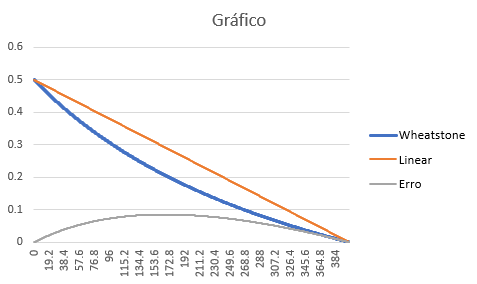
\includegraphics[height=8cm]{./image/PESTA/graph/grafico-1.png}
%		\caption{\textit{Wheatstone} comportamento}
%		\label{wheatstone-reaction}
%	\end{figure}
%\end{minipage}
%\minipagespace{.5}
Esta célula de carga de $50 \; Kg$ tem uma resolução na saída de $2 \; mV$ por cada $1 \; Volt$ da sua alimentação com mais ou menos $0.15 \; mV$ de erro. Isto quer dizer que, se for alimentada com $5 \; V$, esta vai ter na saída uma variação de tensão mínima de $10 \; mV$ e a margem de erro total de leitura está na ordem de mais ou menos $0.03\%$, segundo indicação de seu \textit{datasheet}.
Esta célula de carga tem interferências da temperatura, ruídos e se usada durante longos contínuos períodos de tempo.
\\
\\
Como indicado no \textit{datasheet} o valor obtido pode ter interferência de $0.03\%$ por cada meia hora de utilização, e $0.0016\%$ por cada grau de temperatura em excesso. Convém neste caso manter desligado o equipamento e apenas ser usado quando necessário, ou fazer \textit{offset} tendo em consideração a margem de erro.
\\
\\
%https://www.800loadcel.com/load-cell-and-strain-gauge-basics.html
%Para perceber melhor o funcionamento do sensor \textit{\textbf{strain gauge}} é aconselhável recorrer a literatura \cite{book-9} e \cite{book-10}, que explica como são feitas, seus dimensionamentos e processos de fabrico.
A montagem da mesa (prato) de medição é apresentada na \autoref{Prato}.
%Esta montagem deve ser explicada e a figura deve permitir ver todos os elementos, que devem estar devidamente identiificados
\\
\\
\begin{minipage}[!b]{\linewidth}
\begin{figure}[H]
	\centering
	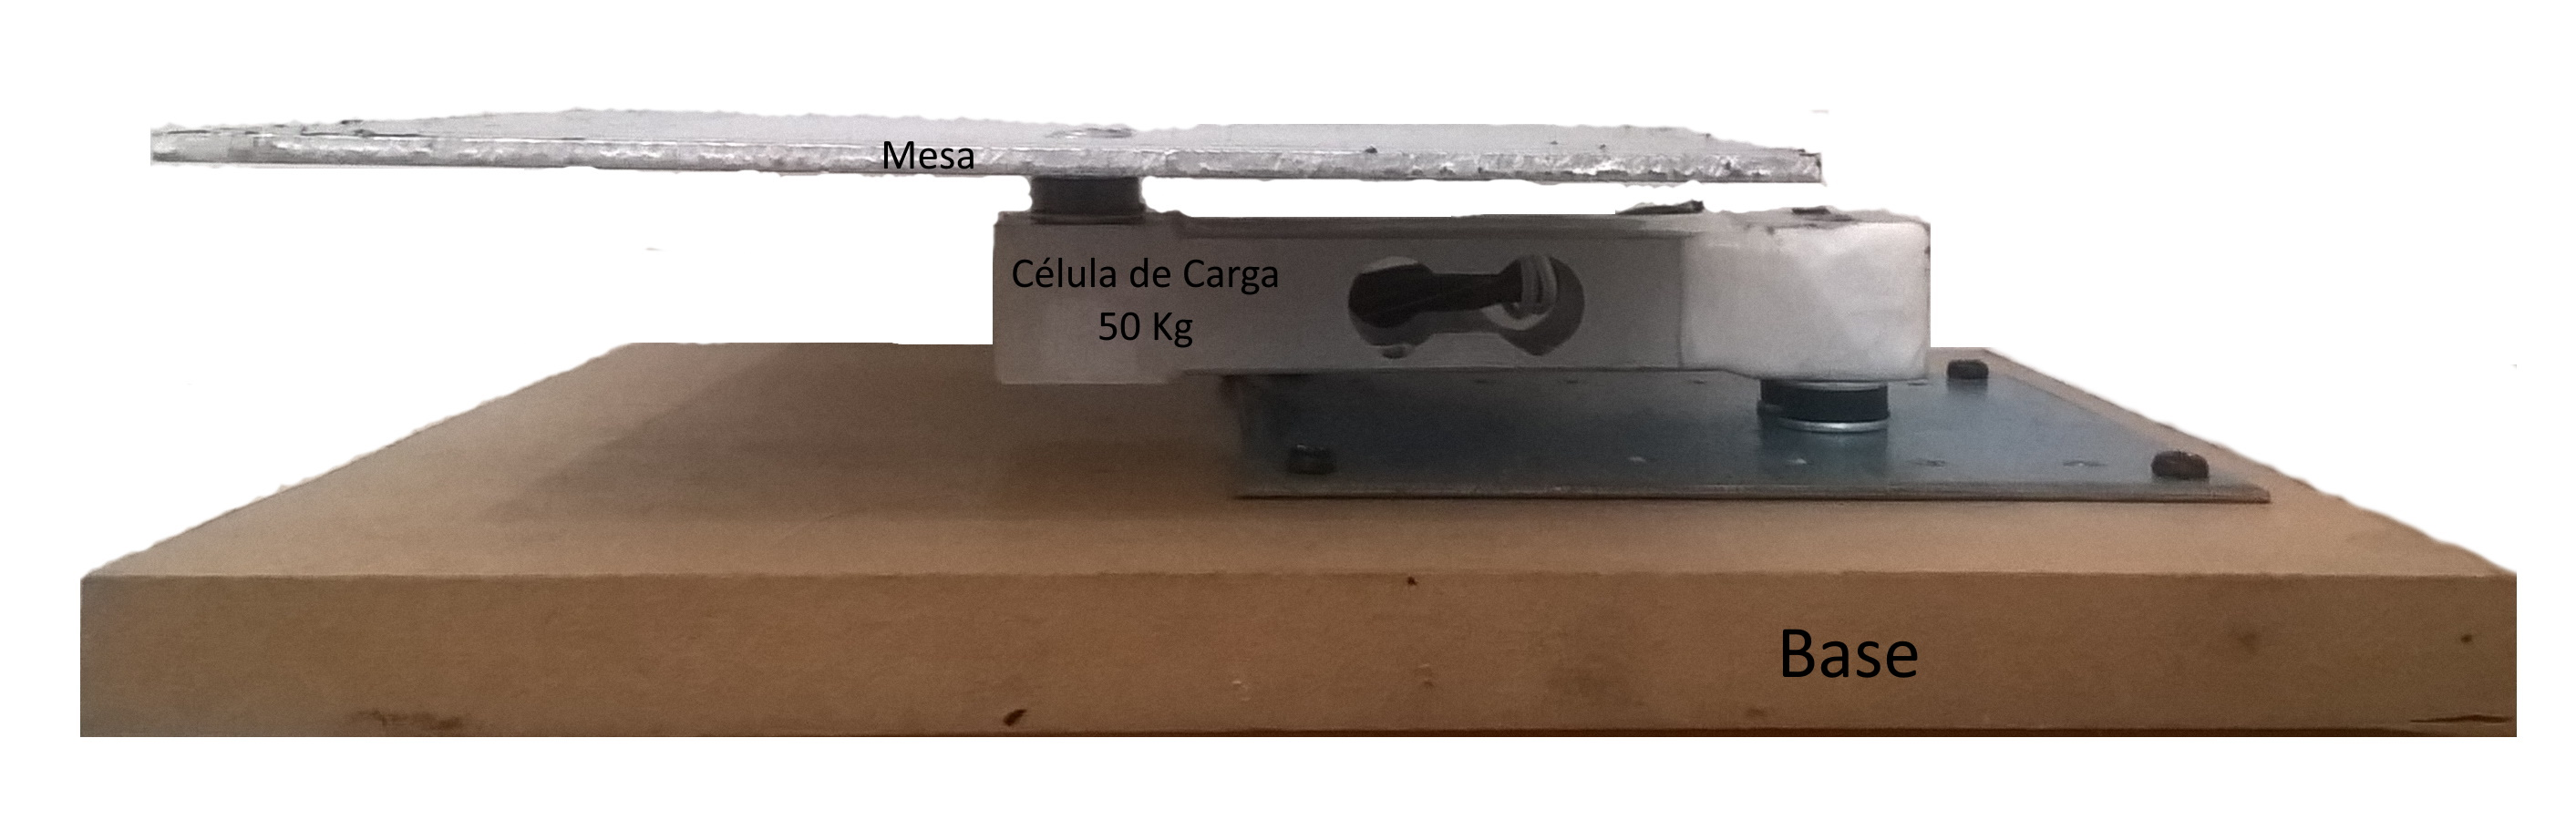
\includegraphics[scale=0.14]{./image/PESTA/material/Prato-1.jpg}
	\caption{Prato}
	\label{Prato}
\end{figure}
\end{minipage}
\minipagespace{.5}
Ao colocar uma massa sobre a mesa, esta vai exercer pressão na célula de carga, que vai resultar numa tensão mecânica e compressão nos sensores \textit{strain gauge} que estão assentes na superfície do corpo da célula de carga, provocando uma diferença de potencial correspondente. Estes sensores não estão visíveis nesta célula de carga porque esta têm uma camada protetora de silicone branco sobre eles.
%%%%%%%%%%%%%%%%%%%%%%%%%%%%%%%%%%%%%%%%%%%%%%%%%%%%%%%%%%
\section{Amplificador de sinal e \acs{adc}}
A amplificação é geralmente um requisito fundamental, pois a maioria dos sensores tende a produzir níveis de sinal significativamente mais baixos do que aqueles usados no processador digital. Os sensores resistivos podem precisar de um amplificador para a célula de carga. Se possível, é vantajoso ter o ganho o mais próximo possível do elemento sensor, eliminado interferências de ruído e da resistência da cablagem. Em situações onde um maior ganho é necessário, muitas vezes pode haver implicações para lidar com quaisquer efeitos adversos, como o ruído, problemas de \textit{layout} do \textit{chip}, e os transitórios agudos associados aos sinais digitais que precisam de ser mantidos bem longe dos circuitos analógicos \textit{front-end}. \cite{book-9}
\\
\\
Neste projeto foi utilizado o HX711, que está apresentado na \autoref{HX711_Schematic_1}. 
\\
\begin{figure}[H]
	%\captionsetup{justification=raggedright,singlelinecheck=false}
	\centering
	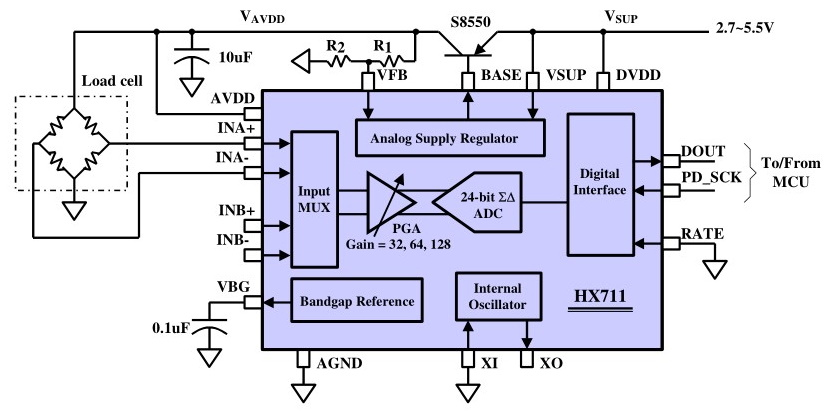
\includegraphics[scale=0.3]{./image/PESTA/schematic/HX711_Schematic_1.jpg}
	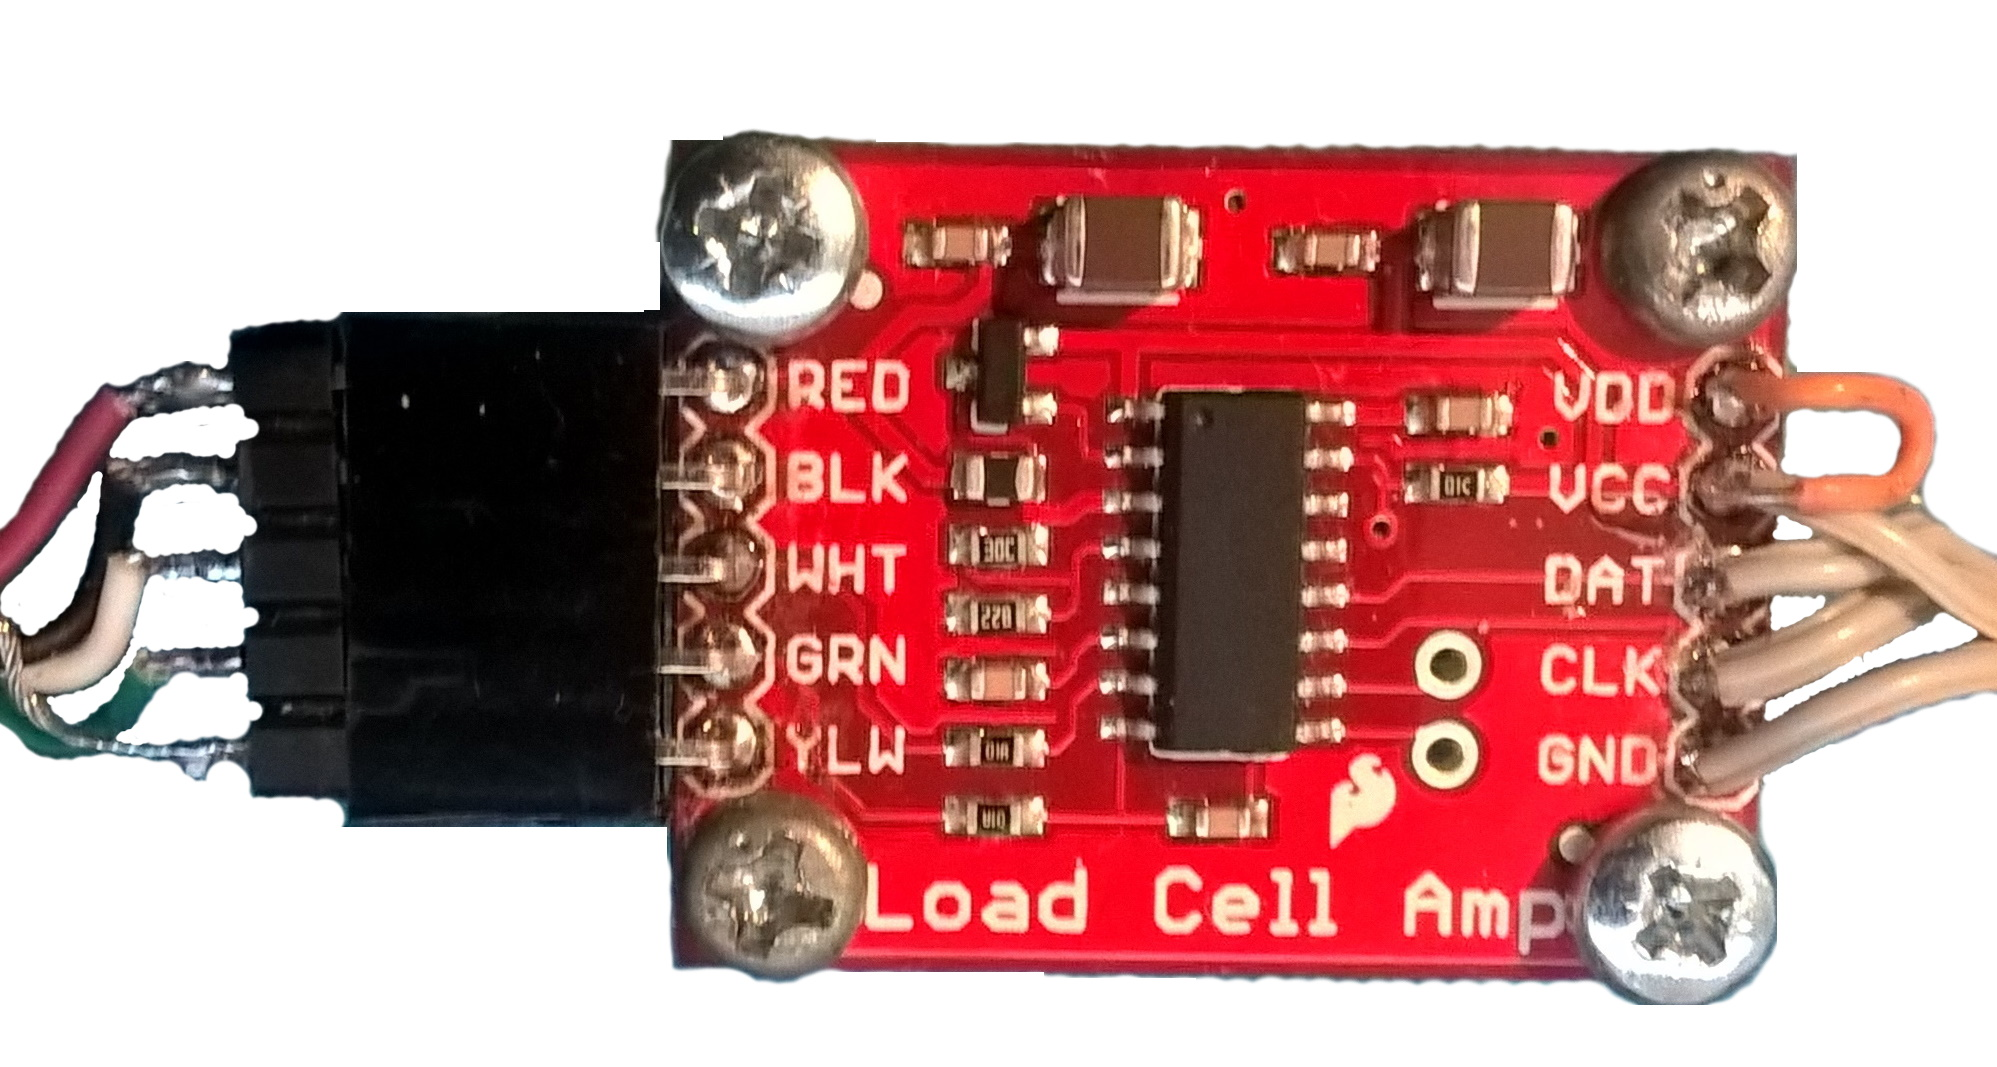
\includegraphics[scale=0.09]{./image/PESTA/material/HX711_board_1.jpg}
	\caption{Esquema de ligações e a placa do HX711}
	\label{HX711_Schematic_1}
\end{figure}
\figurespace{.5}
A ligação deste componente é fácil de se perceber tal como indicado na \autoref{HX711_connection}.
\\
%Então deve ser apresentada
%Apresenatação das figuras e da tabela....
\begin{table}[H]
	\centering
	\caption{Terminais HX711 ({\tiny \scriptsize{top view}})}
	\begin{tabular}{||L{2cm} L{4cm} | p{4cm}  C{2cm}||}
		\hline
		\multicolumn{2}{||c|}{MCU} & \multicolumn{2}{|c||}{\textit{Célula de peso}}\\ [1ex]
		\hline
		1 & GND & EARTH (GND) & YLW \\ 
		2 & CLK & INPA & GRN \\
		3 & DATA & INNA & WHT \\
		4 & VCC &  GND & BLK \\
		5 & VDD & $V_{ADC}$ & RED \\ [1ex]
		\hline
	\end{tabular}	
	\label{HX711_connection}
\end{table}
\tablespace{.5}
 A parte mais complexa neste trabalho é a interligação dos equipamentos com o microcontrolador por meio de \textit{software} e a criação das bibliotecas e os \textit{drivers} de comunicação,
%como a placa do amplificador de célula de carga (\textit{chip} HX711 figura \ref{HX711_Schematic_1}),
 já que o protocolo de comunicação é proprietário. O mesmo está demonstrado na \autoref{Protocolo}.
\\
\\
Pode-se consultar a biblioteca \textit{driver} do amplificador de célula de carga HX711 nos anexos \ref{hx711-h} e \ref{hx711-c}.
\\

%apresentar tabela
%A conversão AD deve ser apresentada... indicar a resolução do peso medido
\begin{figure}[H]
	%\captionsetup{justification=raggedright,singlelinecheck=false}
	\centering
	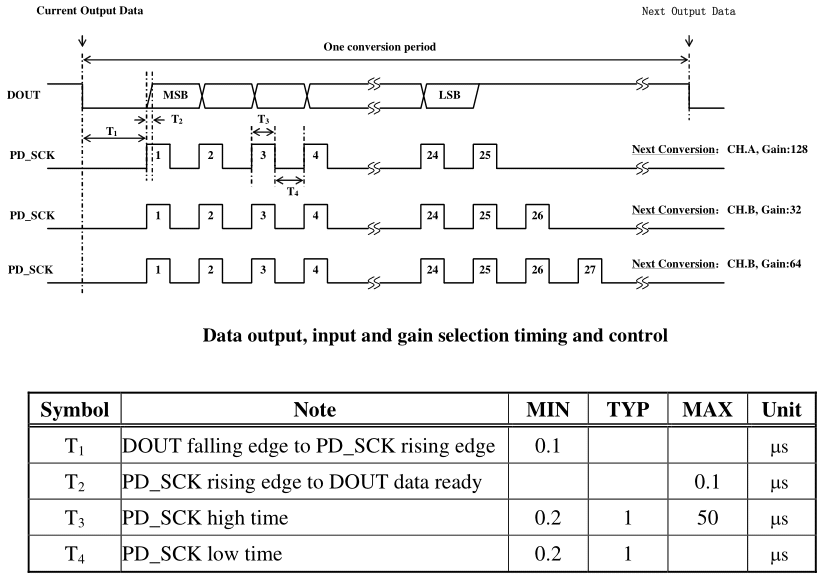
\includegraphics[scale=0.6]{./image/PESTA/comunicacao/Protocolo.png}
	\caption{Protocolo de comunicação}
	\label{Protocolo}
\end{figure}
\figurespace{.3}
A placa 
%\textit{Load Cell Amplifier}
pode ser fisicamente configurada para determinar o número de amostras por segundo a ser transmitido. Este circuito tem duas opções: a opção de 10 amostras por segundo, e de 80 amostras por segundo. Neste projeto foi utilizada a segunda opção, que necessita de uma pequena alteração na placa de circuito de impresso, isto é, é necessário abrir o respetivo \textit{jumper} de configuração.
\\
\\
A conversão de informação acontece na transição entre o sinal contínuo da vida real, para um sinal discreto associado ao mundo digital. Tipicamente esta etapa consiste na conversão de um sinal analógico para digital.\cite{book-9}
\\
O processamento digital pode consistir de rotinas para compensar os desvios por linearização, a sensibilidade e o \textit{offset}, ou o processamento de técnicas mais sofisticadas como reconhecimento de padrões, (tais como, redes neuronais) para equipamentos de sensores vetoriais.\cite{book-9}
\\
A comunicação é responsável por criar rotinas necessárias para transferir e receber a informação e sinais de controle, entre o sensor e o processador, que toma lugar como componente central, tratando a informação, guardando os dados e fazendo rotinas, tais como, de calibração, e de teste e controlo de ganho da amplificação. \cite{book-9}
\\
\\
Abaixo a \autoref{SPS_64} que foi adquirida do trabalho realizado recorrendo ao osciloscópio da RIGOL DS1102E e seu software \textit{Rigol Waveform Viewer}, demonstrando a comunicação entre o amplificador de sinal e o microcontrolador da informação do \acs{adc}, a linha amarela é a informação (\acs{adc}) e a azul os impulsos do \textit{clock} (PD\_SCK). Neste exemplo é visível cinco conversões executadas.
\\
\begin{figure}[H]
	\centering
	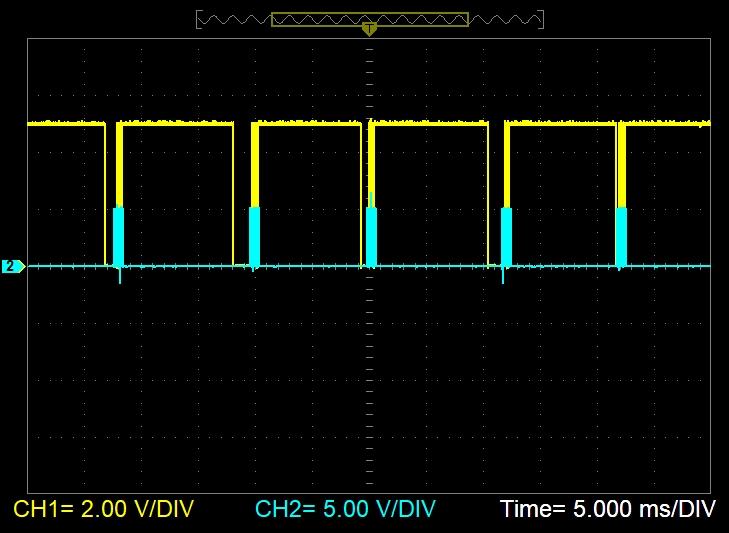
\includegraphics[scale=0.42]{./image/PESTA/graph/80SPS64GAIN/SPS_80.JPG}
	\caption{Amostras}
	\label{SPS_64}
\end{figure}
\figurespace{.5}
A biblioteca (\textit{driver}) do integrado HX711 recorre a interrupções periódicas. Quando a linha de sinal da informação (amarela) vai para a massa esta indica que tem um pacote de leitura pronto a ser transmitido.
\\
\\
\begin{minipage}[!b]{\linewidth}
\begin{minipage}[!b]{.45\linewidth}
	\begin{table}[H]
		\captionsetup{justification=raggedright,singlelinecheck=false}
		\caption{Configuração Ganho}
		\begin{tabular}{ | c | c | c |  }
			\hline
			\makecell[c]{PD\_SCK \\ Impulsos} & Entrada  & Ganho \\
			\hline
			\hline
			25 & \textbf{A} & 128 \\
			\hline
			26 & \textbf{B} & 32 \\
			\hline
			27 & \textbf{A} & 64 \\
			\hline
		\end{tabular}
		\label{Gain_Selection}
	\end{table}
	\tablespace{2.5}
\end{minipage}
\begin{minipage}[l]{.53\linewidth}
\vspace{.1cm}
Como indicado abaixo nos gráficos, em que a linha \textcolor{yellow}{amarela} é a informação e a linha \textcolor{BlueGreen}{azul} o respetivo \textit{clock} que é gerado pelas interrupções do microcontrolador, fazendo um deslocamento dos \textcolor{blue}{24} \textit{bits}, que por fim transmite para o amplificador o ganho de amplificação a ser usado pelo numero excedente de \textit{clock cycles}, em que nesta demonstração da \autoref{Gain_128_example} é \textcolor{blue}{um}, e corresponde a um ganho de \textcolor{blue}{128}, respeitando a informação apresentada na \autoref{Gain_Selection},  e de seguida o exemplo da \autoref{Gain_64_example}, com um ganho de \textcolor{blue}{64}, pois tem \textcolor{blue}{três} impulsos excedentes.
\end{minipage}
\end{minipage}
\\
\\
\begin{minipage}[!b]{\linewidth}
\begin{minipage}[!b]{.43\linewidth}
\begin{figure}[H]
	\captionsetup{justification=raggedright,singlelinecheck=false}
	\flushleft
	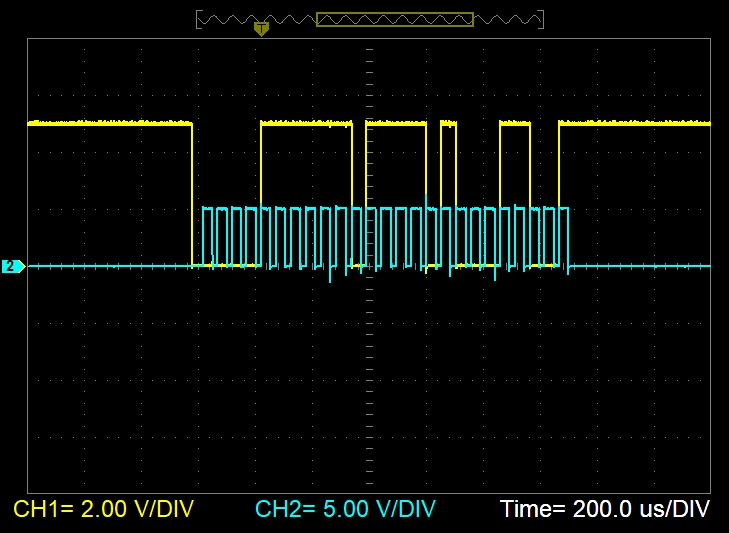
\includegraphics[scale=0.26]{./image/PESTA/graph/80SPS128GAIN/Gain_128_example.JPG}
	\caption{Ganho de 128}
	\label{Gain_128_example}
\end{figure}
\end{minipage}
\hspace{.8cm}
\begin{minipage}[!b]{.43\linewidth}
\begin{figure}[H]
	\captionsetup{justification=raggedright,singlelinecheck=false}
	\flushleft
	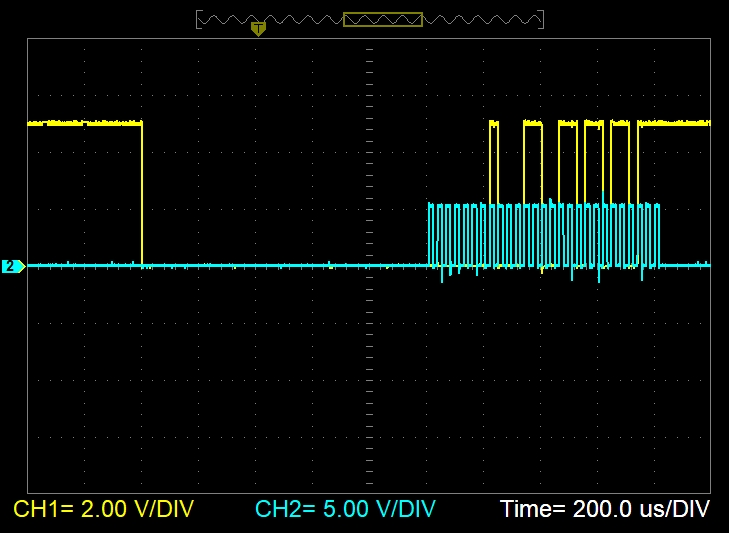
\includegraphics[scale=0.26]{./image/PESTA/graph/80SPS64GAIN/Gain_64_example.JPG}
	\caption{Ganho de 64}
	\label{Gain_64_example}
\end{figure}
\end{minipage}
\end{minipage}
\minipagespace{.5}
Para obter este resultado, a livraria \textit{driver} para o \textit{Load Cell Amplifier} teve de ter em consideração que a arquitetura do microcontrolador é de 8 \textit{bits}, uma vez que a estrutura do pacote de informação é entre 25 a 27 impulsos do \textit{clock cycle} em que é transmitido primeiro o \ac{msb}.
\\
\\
Este amplificador de célula de carga tem uma amplificação no sinal de entrada com valores indicados na \autoref{Gain_Selection}, e tem uma resolução de 24 \textit{bits}, como se sabe os números podem representar quantidades e intervalos, os 24 \textit{bits} representa um intervalo de 0 até \, $2^{24}-1$, que nos dá 16777215 unidades, ou seja, o sinal de entrada amplificado pode ser dividido por este numero, isto é, pode-se obter este número de leituras possíveis, em que, se se tratar por exemplo de 5 Volt pode-se obter 16777215 leituras de intervalos de aproximadamente $2.98 \times 10^{-7}$ Volt cada, uma precisão muito boa.
%%%%%%%%%%%%%%%%%%%%%%%%%%%%%%%%%%%%%%%%%%%%%%%%%%%%%%%%%%
\section{Display \acs{lcd}}
%Porque este ?
%O que pretende que seja visualizado ?
O \ac{lcd} utilizado é de 4x20, isto é, quatro linhas de vinte caracteres cada, tornando-se no interface humano principal, e também durante este projeto numa ferramenta extremamente útil para fazer o \textit{debug} e executar testes ao código pela visualização das informações adversas.\\
Este \acs{lcd} é usado para visualizar as leituras e o valor de calibração da célula de carga, a escolha deste \textit{display} é unicamente por ter este componente no stock existente de material com uma biblioteca que o suporta, uso este de quatro linhas apenas para facilitar a deteção de anomalias ao testar o código visualizando vários parâmetros ao mesmo tempo.
\\
\\
%que projectos ?
%mencionar relatórios e mencionar relatorio LABSIS.
A biblioteca ou driver do \acs{lcd} que já tinha feito para outros projetos pessoais serviu para utilizar na disciplina de laboratório de sistemas \cite{article-1} e neste projeto, poupando bastante tempo, revelando a importância de documentar os conhecimentos adquiridos. A biblioteca está presente no \textit{anexado} \ref{lcd-h} e \ref{lcd-c}.
%[\ref{codigo}]
\\
\\
Abaixo está uma imagem do \acs{lcd} de 4x20 azul na \autoref{4x20_LCD} e na \autoref{LCD_connections}, suas respetivas ligações.
\\
\begin{figure}[H]
	\centering
	%%\captionsetup{justification=raggedright,singlelinecheck=false}
	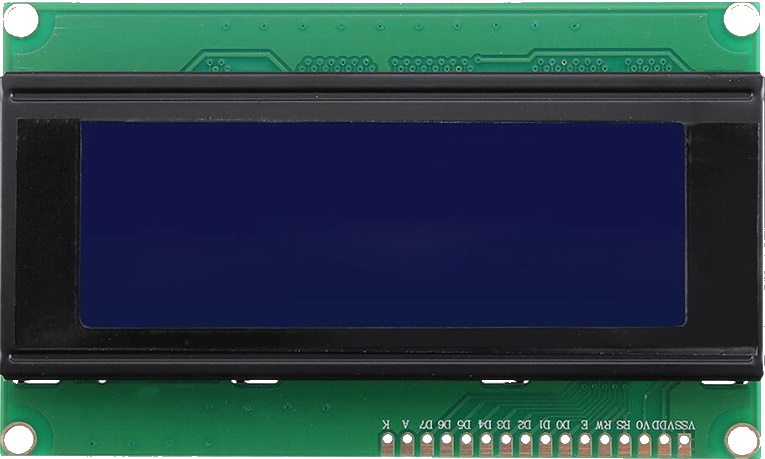
\includegraphics[height=6cm]{./image/PESTA/material/4x20_LCD.jpg}
	\caption{\acs{lcd}}
	\label{4x20_LCD}
\end{figure}
\begin{table}[H]
	\centering
	\caption{Ligações \acs{lcd}}
	\begin{tabular}{||p{1cm} p{2cm} p{4cm} | p{1cm}||} 
		\hline
		\multicolumn{3}{||c|}{\textbf{LCD Pin}} & \multicolumn{1}{|c||}{\textbf{MCU Pin}}\\ [1ex]
		\hline
		1 & VSS & GND & \\
		2 & VCC & +5V & \\
		3 & VEE & \textit{Contrast Control} & \\
		4 & RS & \textit{Register Select} & Pin 0 \\
		5 & RW & \textit{Read/Write} & Pin 1 \\
		6 & E & \textit{Enable} & Pin 2 \\
		7 & Do & \textit{Data Pin 0} & \\
		8 & D1 & \textit{Data Pin 1} & \\
		9 & D2 & \textit{Data Pin 2} & \\
		10 & D3 & \textit{Data Pin 3} & \\
		11 & D4 & \textit{Data Pin 4} & Pin 4 \\
		12 & D5 & \textit{Data Pin 5} & Pin 5 \\
		13 & D6 & \textit{Data Pin 6} & Pin 6 \\
		14 & D7 & \textit{Data Pin 7} & Pin 7 \\
		15 & LED+ & \textit{Led +5V} &  \\
		16 & LED- & \textit{Led Ground} & \\
		\multicolumn{3}{||c|}{\textit{Reboot} \acs{lcd}} & \multicolumn{1}{|l||}{Pin 3}\\ [1ex]
		\hline
	\end{tabular}
	\label{LCD_connections}
\end{table}
%%%%%%%%%%%%%%%%%%%%%%%%%%%%%%%%%%%%%%%%%%%%%%%%%%%%%%%%%%
\section{Microcontrolador}
Os microcontroladores da Atmel de 8 a 32 \textit{bits} são baseados na arquitetura avançada de Harvard, na qual está concebido para baixo consumo e alta performance.
\\
\\
Este tipo de arquitetura tem dois \textit{buses} (barramentos), um dedicado à leitura das instruções a executar e outro para a escrita e leitura de dados (informação ou dados), isto assegura que uma nova instrução pode ser executada em cada ciclo de relógio, em que elimina todos os estados de espera, quando não há instruções prontas a executar.
\\
\\
Nos microcontroladores do \ac{avr}, os barramentos estão configurados de forma a dar prioridade ao barramento das instruções do \ac{cpu} acesso à memória flash, enquanto o barramento da \acs{cpu} de dados tem prioridade de acesso à \ac{sram}.
\\
\\
O espaço de memória de dados é dividido em três partes, os \ac{gpr} as \ac{sfr} ou memória de I/O e a \textit{data} \acs{sram}.
\\
\\
Os microcontroladores da \acs{avr} utilizam uma arquitetura de instruções \ac{risc} que reduz a complexidade dos circuitos na codificação de cada instrução. Daí que os microcontroladores que se baseiam nestes tipos de arquitetura são sinónimo de código reduzido, alta performance e baixo consumo energético.
\\
\begin{figure}[H]
	\centering
	%%\captionsetup{justification=raggedright,singlelinecheck=false}
	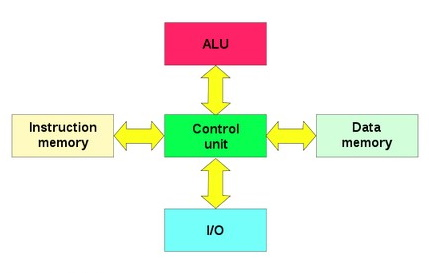
\includegraphics[scale=1]{./image/PESTA/Diagrama/Harvard_architecture.jpg}
	\caption{Harvard Architecture}
	\label{Harvard_architecture}
	\vspace{.1cm}
	\qquad link: \url{https://en.wikipedia.org/wiki/Harvard_architecture}
\end{figure}
\figurespace{.5}
%\qquad link: \url{https://en.wikipedia.org/wiki/Harvard_architecture}
%Porque esta opção?
%O facto de ser um dos masi poderosos.. não é justificação
%A seleção do material deve ser justificada de forma mais citeriosa
%Devia ser feita uma pesquisa de produtos e seleção baseada nos requisitos prédefinidos.
O Atmega 128 (\autoref{Atmega_128_pinagem}) é um dos mais poderosos \ac{mcu} da linha de 8 \textit{bits} da Atmel, e neste projeto esta integrado numa placa de desenvolvimento dotado de ligações por fichas \ac{idc}, ou seja, utiliza \textit{flat ribbon cables} para ligar os periféricos, o que é muito mais prático do que sistemas que atualmente são mais populares, como por exemplo a placa de desenvolvimento Arduino, STMicroelectronics e a \ac{pic} que recorrem a um interface por pinos (\textit{pin headers}).
\\
\begin{figure}[H]
	\centering
	%%\captionsetup{justification=raggedright,singlelinecheck=false}
	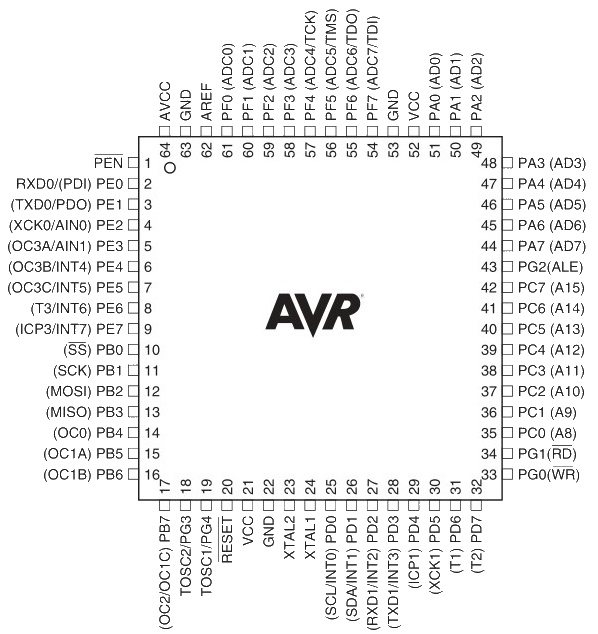
\includegraphics[scale=0.5]{./image/PESTA/material/Atmega128_1.jpg}
	\caption{Atmega 128}
	\label{Atmega_128_pinagem}
\end{figure}
\figurespace{.5}
%{Transparências Sistemas Digitais 2 \quad \acs{isep} \quad 2008/2009 \quad \textit{link}}: \\
%\url{https://drive.google.com/file/d/1wgOGf8WwYY0OzDhRca9ypXz-iBO55YOF/view?usp=sharing} \\ \\
Esta opção preenche os requisitos requeridos, por ter portas de entrada e saída suficientes, porque o \acs{lcd} requer a utilização de oito pinos para funcionar, o amplificador de célula de carga dois pinos, temos quatro botões que requer quatro pinos de entrada e três \textit{leds} indicadores, ou seja, três pinos de saída. Por aqui deduzimos que o \acs{mcu} a escolher tem que ter mais do que dezasseis pinos só para os periféricos.
\\
O \acs{mcu} também tem que ter dois temporizadores capazes de gerar os tempos desejados por interrupções, talvez seria possível fazer isto com um micro controlador com menos capacidades, porque este projeto não utiliza a funcionalidade do \acs{adc} nem comunicações série integradas, no entanto comparando a nível de preço com as alternativas destaca-se esta opção.
\\
\\
Alternativas que foram postas em consideração estão na \autoref{Boards-1}, e foram excluídas pelos motivos mencionados.
\\
\begin{figure}[H]
	\centering
	%%\captionsetup{justification=raggedright,singlelinecheck=false}
	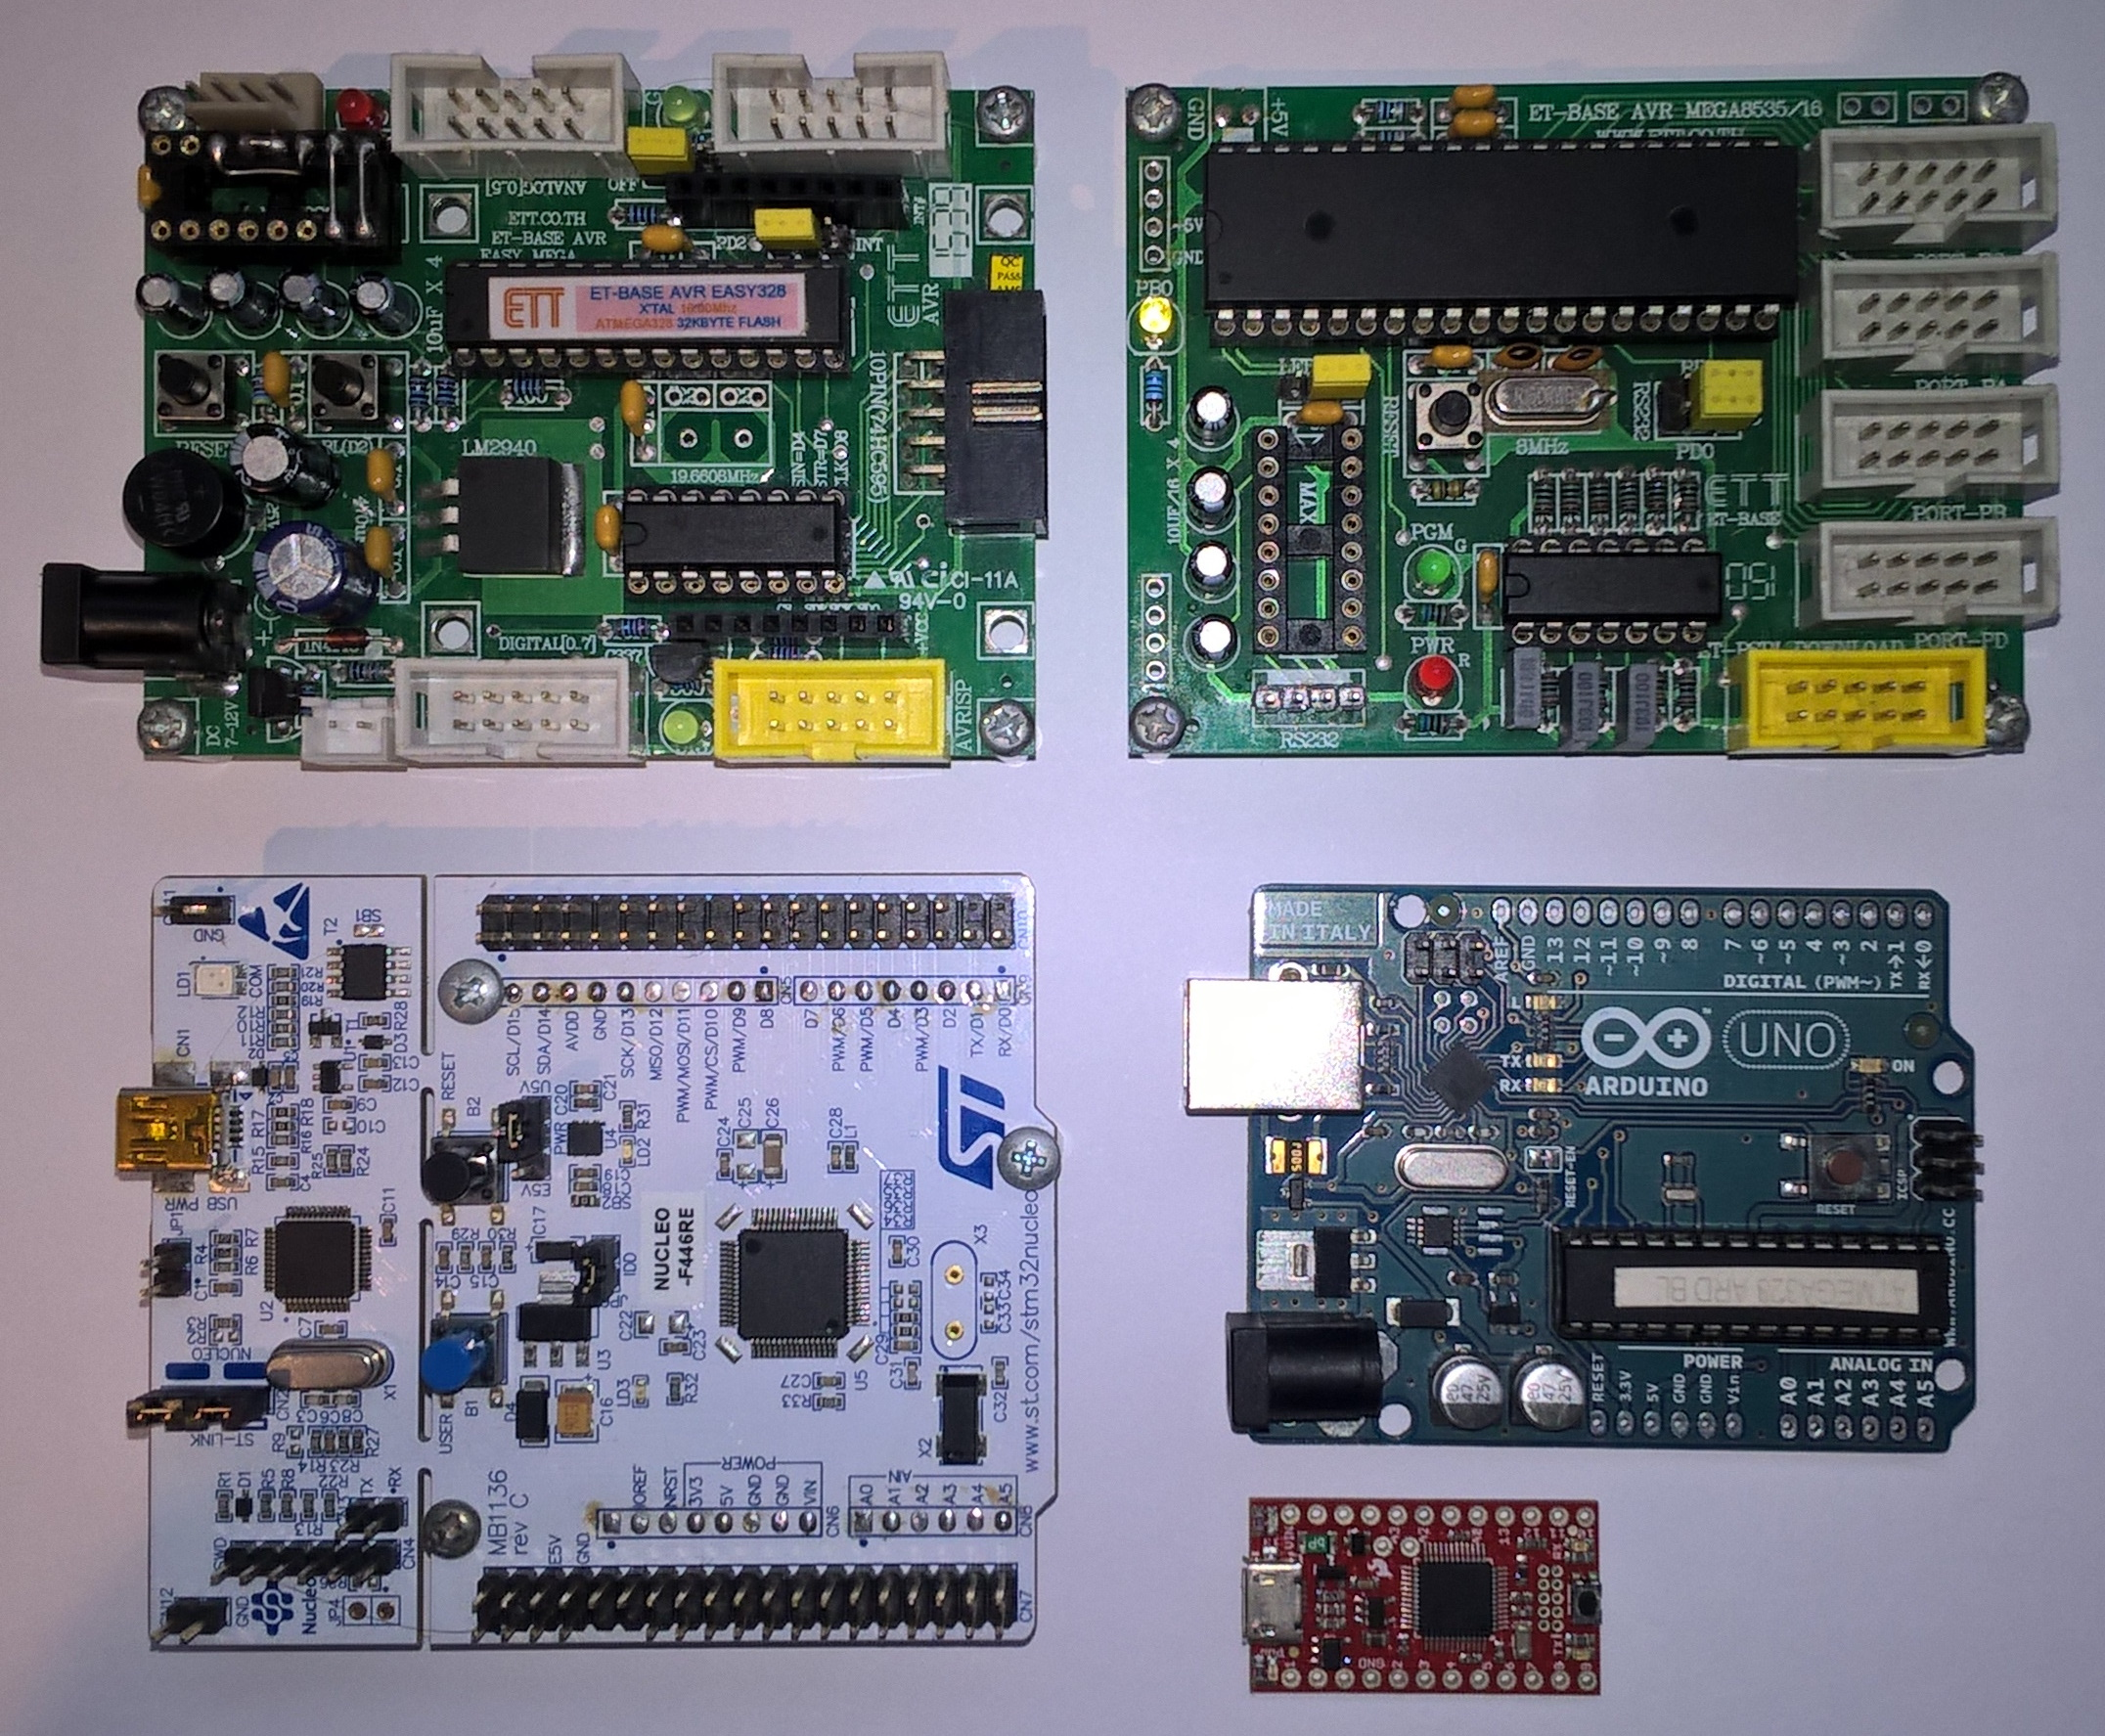
\includegraphics[scale=0.17]{./image/PESTA/boards/Boards-2.jpg}
	\caption{Alternativas ao Atmega 128}
	\label{Boards-1}
\end{figure}
\figurespace{.5}
Dos componentes que constituem o Atmega 128, os temporizadores são os que considero os mais importantes devido a ser uma das grandezas fundamentais, o tempo, podendo este gerar intervalos de tempo e \acp{pwm}
%porque
, o \ac{adc} do \acs{mcu} nem vai ser usado neste projeto, vai ser utilizado um \textit{load cell amplifier} externo, uma alternativa que é muito melhor porque tem maior resolução e específico para a aplicação em causa.
\\
\\
Talvez os \acsp{mcu} nem deviam ter a componente \acs{adc} e realçar em meios de comunicação e memoria, tornava-se assim num sistema unicamente digital.
O Atmega 128 é uma escolha acertada para este projeto, considerando as alternativas de optar por um \ac{mcu} de 32 \textit{bits} ou um \textit{embedded system} com sistema operativo integrado, em que no primeiro caso o grau de dificuldade é acrescida devido a ter muito mais configurações e funcionalidades, e a segunda opção de ser exagerada, devido a só utilizar uma muito pequena parte das suas possibilidades, como se diz em inglês um \textit{overkill}, desperdiçando recursos desnecessariamente, e também se iria refletir a nível de custos monetários, no entanto facilita bastante no desenvolvimento de qualquer projeto, pois estaria-se a trabalhar sobre uma camada de nível superior (\textit{Kernel}).
\\
\\
\begin{minipage}{\linewidth}
%{\Large Características do Atmega 128 :}
As características do microcontrolador Atmega 128 :
\normalsize
\begin{itemize}	
	\setlength\itemsep{-0.3em}
	\item Arquitectura \acs{risc}
	\item 33 instruções (a maior parte executada num único ciclo de execução)
	\item 32 x 8 registos de trabalho (arquitectura de registos)
	\item Até 16 \acs{mips} (@16MHz) – 62.5ns / instrução
	\item 64K x 16 palavras de programa – 128K bytes FLASH
	\item 4K bytes de \acs{ram} interna
	\item 4K bytes de E2PROM de dados
	\item Ciclos de escrita / leitura – FLASH=10000, E2PROM=100000
	\item 7 Portos de IO \\
		\hspace*{.5cm}	-> 6 x 8 bits (Portos A .. F) \\
		\hspace*{.5cm}	-> 1 x 5 bits (Porto G)
	\item 2 x Timer / Counter de 8 bits
	\item 2 x Timer / Counter de 16 bits
	\item 1 x Real Time Counter ( com oscilador independente)
	\item 2 x \acs{pwm} de 8 bits
	\item 6 x \acs{pwm} de 16 bits
	\item \acs{adc} de 10 bits (8 canais)
	\item 2 x \acs{usart}
	\item \acs{spi}
	\item \acs{twi} (I2C)
\end{itemize}
\end{minipage}
\minipagespace{.5}
Para programar este microcontrolador (\textbf{Atmega 128}), foi utilizado o programador da marca da Atmel, o \ac{atmel-ice} \autoref{Programador_1}. Para este equipamento tem disponível programação via \ac{isp} \autoref{ISP_6_8_10pin} e \ac{jtag}.
\minipagespace{.2}
\begin{minipage}[!b]{.5\linewidth}
	\begin{figure}[H]
		\captionsetup{justification=raggedright,singlelinecheck=false}
		\flushleft
		\includegraphics[scale=0.75]{./image/PESTA/programador/Atmel_ice.png}
		\caption{KIT \acs{atmel-ice}}
		\label{Programador_1}
	\end{figure}
\end{minipage}
\hspace{.5cm}
\begin{minipage}[!b]{.5\linewidth}
	\begin{figure}[H]
		\captionsetup{justification=raggedright,singlelinecheck=false}
		\flushleft
		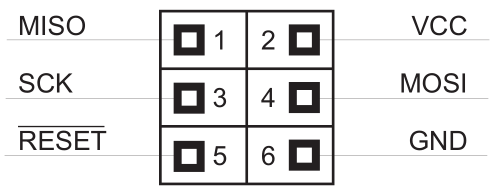
\includegraphics[scale=0.45]{./image/PESTA/programador/isp_6pin.png}
		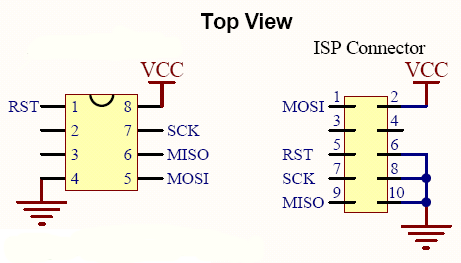
\includegraphics[scale=0.5]{./image/PESTA/programador/isp_8e10pin.png}
		\caption{Fichas \acs{isp}}
		\label{ISP_6_8_10pin}
	\end{figure}
\end{minipage}
\minipagespace{.5}
%%%%%%%%%%%%%%%%%%%%%%%%%%%%%%%%%%%%%%%%%%%%%%%%%%%%%%%%%%
\section{Fonte de Alimentação}
%Introdução a fonte de alimentação...
Está se a usar uma fonte de alimentação comutada abaixadora \autoref{buck-converter}, ou seja, a tensão na sua saída é sempre inferior a da sua entrada e tem uma eficiência até $96\%$.
\\
\begin{minipage}[!b]{.5\linewidth}
	\begin{figure}[H]
		\captionsetup{justification=raggedright,singlelinecheck=false}
		\flushleft
		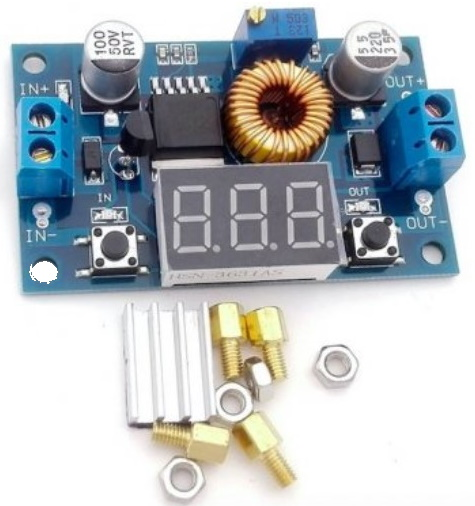
\includegraphics[scale=0.5]{./image/PESTA/material/DCDC_converter.jpg}
		\caption{\textit{Buck Converter}}
		\label{buck-converter}
	\end{figure}
	\figurespace{.1}
\end{minipage}
\begin{minipage}[!b]{.5\linewidth}
\small
Características DC/DC:
	\begin{itemize}
		\setlength\itemsep{-0.5em}
		\footnotesize
		\item 5A 75W Conversor Abaixador (\textit{Step-down})
		\item Alimentação Entrada: 4 - 38VDC
		\item Tensão de saída: 1.25 - 36VDC
		\item Corrente saída: 0 - 5A
		\item Potência saída: 75W
		\item Voltímetro: 4 até 40V, erro ±0.1V
		\item \textit{Led} indicadores
		\item Frequência de operação: 180KHz
		\item Eficiência até 96 \%
		\item Proteção Térmica
		\item Limitador de Corrente
		\item Proteção contra curto circuito
		\item NOTA: Não tem proteção de inversão de polaridade
		\item L x W x H = 6.6 x 3.9 x 1.8 CM
		\item Massa: 28g
	\end{itemize}
\end{minipage}
\minipagespace{.5}
Como a \textit{mainboard} tem um regulador de tensão linear de $5 \; Volt$, para aumentar a eficiência e ter uma alimentação variável de entrada até $38 \; VDC$ foi utilizado o \textit{buck converter} para alimentar o regulador de tensão linear para um valor próximo dos $5 \; Volt$, por exemplo $9 \; Volt$, porque se sabe que as perdas de um regulador de tensão linear é proporcional a queda de tensão entre a sua entrada e a sua saída. Podia-se remover o regulador de tensão linear e apenas utilizar o \textit{buck converter} regulado para o valor de $5 \; Volt$ mas pretende-se não alterar o \acs{pcb} da \textit{mainboard}.
%Explicar melhor
%%%%%%%%%%%%%%%%%%%%%%%%%%%%%%%%%%%%%%%%%%%%%%%%%%%%%%%%%%
\section{Orçamento do material}
Abaixo na \autoref{Material-1}, é apresentado a lista do material utilizado no projeto, bem como o seu preço.
\\
%O orçamento deve estar num anexo, ou no capítulo da apresentação dos componentes, não na validação
\begin{table}[H]{
		\caption{Lista de material}
		\rowcolors{3}{blue!80!yellow!50}{blue!70!yellow!40}
		\begin{tabular}{ |p{9cm}|c|p{2cm}|  }
			\hline
			\multicolumn{3}{|c|}{Lista de Material} \\
			\hline
			Peça & Quant & Preço [uni] \\
			\hline
			Fonte de alimetação 12V 1A & 1 & \EUR{3.87} \\
			Conversor DC-DC com voltímetro & 1 & \EUR{7.75} \\
			ET BASE AVR Atmega128 Board & 1 & \EUR{23.92} \\
			Test Input Board  & 1 & \EUR{3.71} \\
			Test Output Board & 1 & \EUR{3.71} \\
			\acs{idc} Socket 10 way    & 12 & \EUR{0.31} \\
			\acs{idc} Header Straight 10 way    & 12 & \EUR{0.25} \\
			Flatcable    & ? & \EUR{?} \\
			20x4 \acs{lcd} Module Blue & 1 & \EUR{12.24} \\
			SparkFun Load Cell Amplifier HX711 & 1 & \EUR{13.04}   \\
			50Kg Load Cell & 1 & \EUR{12} \\
			\hline
			& \textit{total} & \EUR{86.96} \\
			\hline
		\end{tabular}
		\label{Material-1}
	}
\end{table}
\tablespace{.5}
Os preços são o que estão disponíveis no mercado. Quanto a \textit{mainboard}, o preço do \acs{mcu} Atmega 128 foi o mais competitivo. Outras alternativas, de \acs{mcu} de igual ou menor capacidade, atingiam o mesmo preço ou até seriam mais caras.
%%%%%%%%%%%%%%%%%%%%%%%%%%%%%%%%%%%%%%%%%%%%%%%%%%%%%%%%%%
